\documentclass[border=8pt]{standalone}
\usepackage{tikz}
\usetikzlibrary{arrows.meta, positioning, calc}

% Persona accent colours (Okabe-Ito, colourblind-safe)
\definecolor{maximiser}{HTML}{0072B2}    % blue
\definecolor{understander}{HTML}{009E73}  % teal
\definecolor{finisher}{HTML}{D55E00}      % vermillion
\definecolor{anxious}{HTML}{CC79A7}        % rose
\definecolor{juggler}{HTML}{E69F00}        % orange
\definecolor{weekblue}{HTML}{56B4E9}      % sky

% Colours matched to the light site palette (Catppuccin Latte)
\colorlet{txtmain}{black}
\colorlet{txtmuted}{black!55}
\colorlet{cardfill}{white}
\definecolor{cardborder}{HTML}{CCCCCC}
\colorlet{cardtext}{black!75}
\colorlet{flowfill}{weekblue!8}
\colorlet{flowtext}{black}

\begin{document}
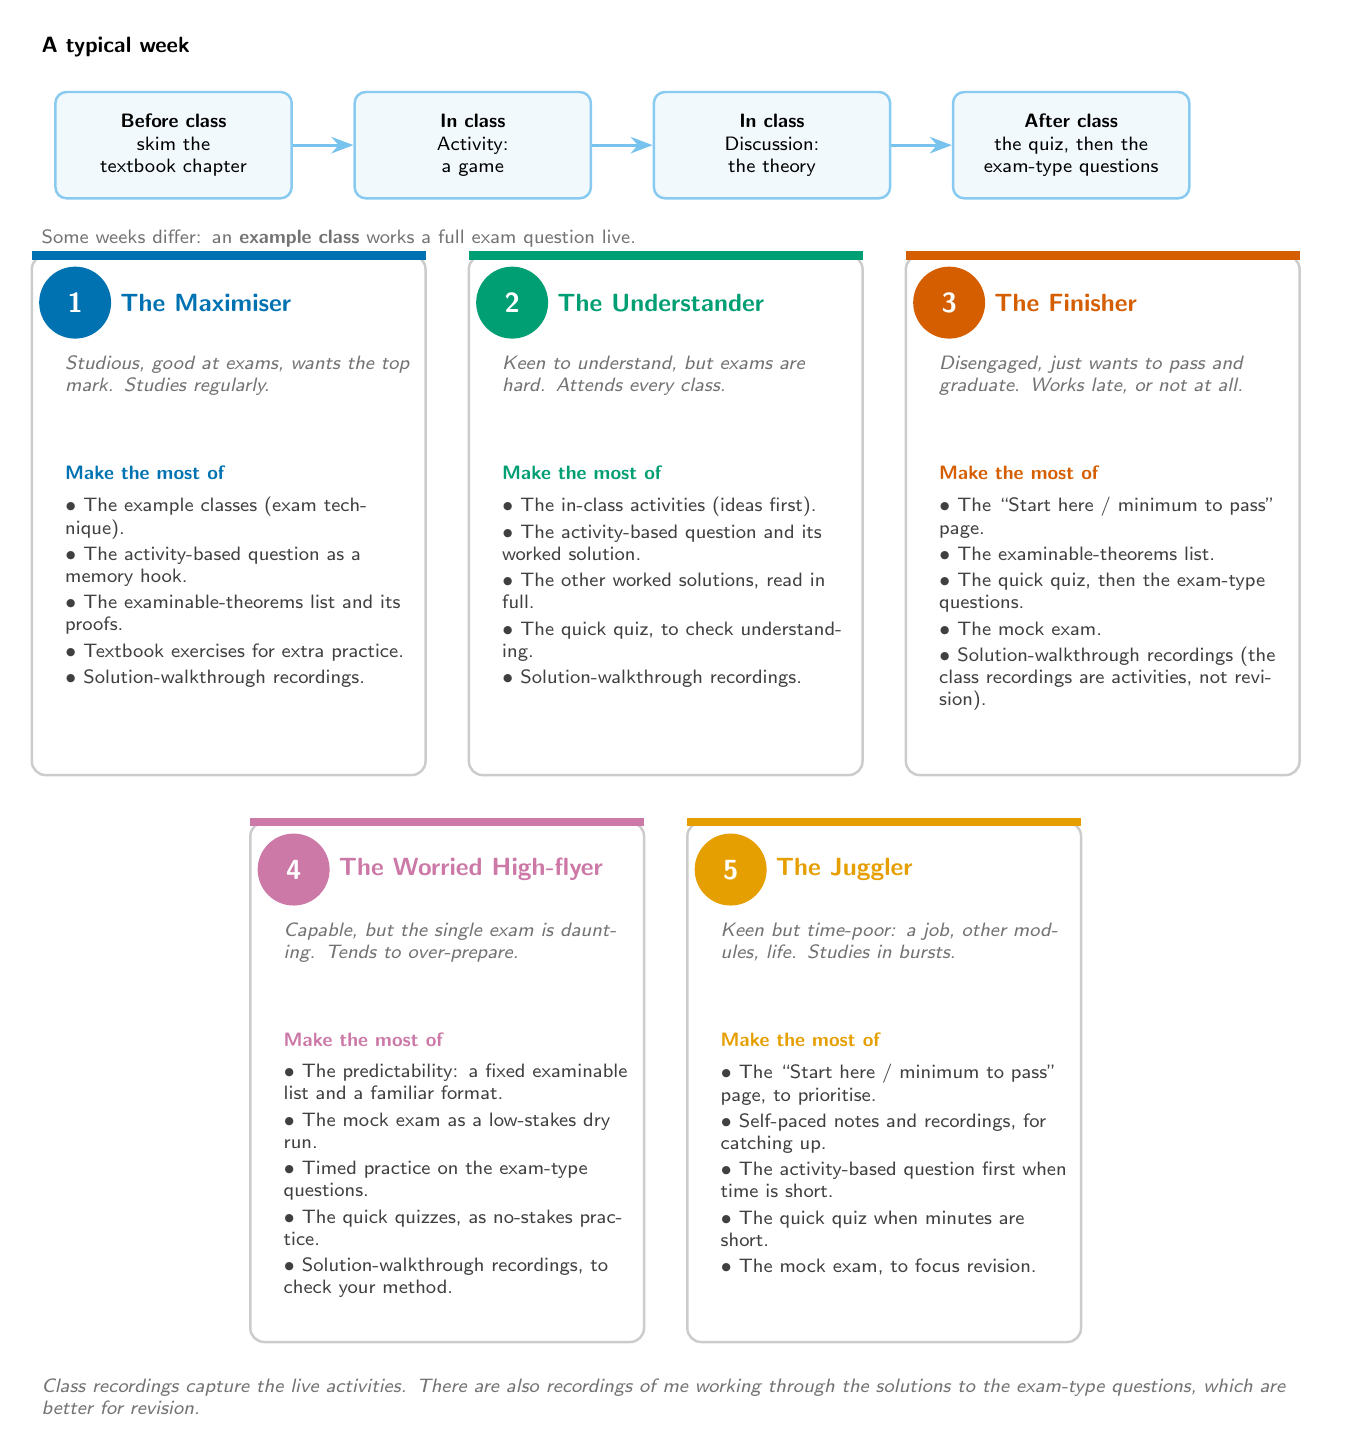
\begin{tikzpicture}[
    font=\sffamily,
    >=Stealth,
    icon/.style={circle, minimum size=26pt, inner sep=0pt, text=white,
                 font=\sffamily\normalsize\bfseries},
    ptitle/.style={font=\sffamily\small\bfseries, anchor=west},
    pdesc/.style={font=\sffamily\scriptsize\itshape, text=txtmuted,
                  align=left, text width=4.4cm, anchor=north west},
    head/.style={font=\sffamily\scriptsize\bfseries, anchor=north west},
    item/.style={font=\sffamily\scriptsize, text=cardtext,
                 align=left, text width=4.4cm, anchor=north west},
    flowbox/.style={rounded corners=4pt, draw=weekblue!70, line width=0.9pt,
                    fill=flowfill, minimum width=3.0cm, minimum height=1.35cm,
                    align=center, font=\sffamily\scriptsize, inner sep=3pt,
                    text=flowtext},
    flowarr/.style={->, line width=1.1pt, weekblue!80},
    flowhead/.style={font=\sffamily\footnotesize\bfseries\itshape, anchor=west,
                     text=txtmain},
    flownote/.style={font=\sffamily\scriptsize, text=txtmuted, align=left,
                     anchor=north west, text width=16.0cm},
]

\def\pw{5.0}
\def\ph{6.6}
\def\gap{0.55}
\def\rowtwo{0}
\def\rowone{7.2}

% ── Persona card macro: #1 x, #2 y, #3 colour, #4 num, #5 title,
%    #6 descriptor, #7 heading, #8 items ──
\newcommand{\personacard}[8]{
    \begin{scope}[shift={(#1, #2)}]
        \draw[rounded corners=5pt, draw=cardborder, line width=0.9pt, fill=cardfill]
            (0, 0) rectangle (\pw, \ph);
        \draw[#3, line width=3pt, rounded corners=5pt]
            (0.0, \ph) -- (\pw, \ph);
        \node[icon, fill=#3] at (0.55, \ph-0.6) {#4};
        \node[ptitle, text=#3] at (1.0, \ph-0.6) {#5};
        \node[pdesc] at (0.3, \ph-1.15) {#6};
        \node[head, text=#3] at (0.3, \ph-2.55) {#7};
        \node[item] at (0.3, \ph-2.95) {#8};
    \end{scope}
}

% ════════════════════════════════════════════════════════════
% TOP BAND: A typical week (flowchart)
% ════════════════════════════════════════════════════════════
\def\wy{15.2}

\node[flowhead] at (0.0, \wy+1.25) {A typical week};

\node[flowbox] (w1) at (1.8, \wy) {\textbf{Before class}\\skim the\\textbook chapter};
\node[flowbox] (w2) at (5.6, \wy) {\textbf{In class}\\Activity:\\a game};
\node[flowbox] (w3) at (9.4, \wy) {\textbf{In class}\\Discussion:\\the theory};
\node[flowbox] (w4) at (13.2, \wy) {\textbf{After class}\\the quiz, then the\\exam-type questions};

\draw[flowarr] (w1) -- (w2);
\draw[flowarr] (w2) -- (w3);
\draw[flowarr] (w3) -- (w4);

\node[flownote] at (0.0, \wy-0.95)
    {Some weeks differ: an \textbf{example class} works a full exam question
     live.};

% ════════════════════════════════════════════════════════════
% TOP ROW of personas
% ════════════════════════════════════════════════════════════
\personacard{0}{\rowone}{maximiser}{1}{The Maximiser}
    {Studious, good at exams, wants the top mark. Studies regularly.}
    {Make the most of}
    {%
        $\bullet$ The example classes (exam technique).\\[1.5pt]
        $\bullet$ The activity-based question as a memory hook.\\[1.5pt]
        $\bullet$ The examinable-theorems list and its proofs.\\[1.5pt]
        $\bullet$ Textbook exercises for extra practice.\\[1.5pt]
        $\bullet$ Solution-walkthrough recordings.%
    }

\personacard{\pw+\gap}{\rowone}{understander}{2}{The Understander}
    {Keen to understand, but exams are hard. Attends every class.}
    {Make the most of}
    {%
        $\bullet$ The in-class activities (ideas first).\\[1.5pt]
        $\bullet$ The activity-based question and its worked solution.\\[1.5pt]
        $\bullet$ The other worked solutions, read in full.\\[1.5pt]
        $\bullet$ The quick quiz, to check understanding.\\[1.5pt]
        $\bullet$ Solution-walkthrough recordings.%
    }

\personacard{2*\pw+2*\gap}{\rowone}{finisher}{3}{The Finisher}
    {Disengaged, just wants to pass and graduate. Works late, or not at all.}
    {Make the most of}
    {%
        $\bullet$ The ``Start here / minimum to pass'' page.\\[1.5pt]
        $\bullet$ The examinable-theorems list.\\[1.5pt]
        $\bullet$ The quick quiz, then the exam-type questions.\\[1.5pt]
        $\bullet$ The mock exam.\\[1.5pt]
        $\bullet$ Solution-walkthrough recordings (the class recordings are activities, not revision).%
    }

% ════════════════════════════════════════════════════════════
% BOTTOM ROW of personas (two cards, centred)
% ════════════════════════════════════════════════════════════
\personacard{2.775}{\rowtwo}{anxious}{4}{The Worried High-flyer}
    {Capable, but the single exam is daunting. Tends to over-prepare.}
    {Make the most of}
    {%
        $\bullet$ The predictability: a fixed examinable list and a familiar format.\\[1.5pt]
        $\bullet$ The mock exam as a low-stakes dry run.\\[1.5pt]
        $\bullet$ Timed practice on the exam-type questions.\\[1.5pt]
        $\bullet$ The quick quizzes, as no-stakes practice.\\[1.5pt]
        $\bullet$ Solution-walkthrough recordings, to check your method.%
    }

\personacard{8.325}{\rowtwo}{juggler}{5}{The Juggler}
    {Keen but time-poor: a job, other modules, life. Studies in bursts.}
    {Make the most of}
    {%
        $\bullet$ The ``Start here / minimum to pass'' page, to prioritise.\\[1.5pt]
        $\bullet$ Self-paced notes and recordings, for catching up.\\[1.5pt]
        $\bullet$ The activity-based question first when time is short.\\[1.5pt]
        $\bullet$ The quick quiz when minutes are short.\\[1.5pt]
        $\bullet$ The mock exam, to focus revision.%
    }

% ── Footer note ──
\node[font=\sffamily\scriptsize\itshape, text=txtmuted, anchor=north west,
      text width=16.1cm]
    at (0, -0.35)
    {Class recordings capture the live activities. There are also recordings of
     me working through the solutions to the exam-type questions, which are
     better for revision.};

\end{tikzpicture}
\end{document}
